\chapter{Measurements}\label{sec:measurements}
This chapter aims to validate the accuracy of force estimation from sEMG after different processing techniques by comparing it to measured data. The goal is to measure sEMG from biceps and triceps,  record the sEMG reference noise and to measure the estimated force using a load cell during an exercise of isometric contraction. The sEMG data is then processed using the different techniques that are discussed in the simulation chapter, and the final estimated force will be compared to the measured force. 

\section{Experimental setup}
The measurement setup consists of the following components:
\begin{itemize}
    \item Siemens Single Point Load Cell, 20kg Range, Compression Measure
    \item Keysight E3631A DC power supply at 2V to power the load cell
    \item TMSi Refa8-16e 16 channel amplifier
    \item Kendall H124SG Foam-Hydrogel ECG Electrodes 
\end{itemize}

The 16 channel amplifier performs uni-polar measurements. This means that each electrode is connected to its own amplifier channel, and the measured values are compared to the value of a reference. The opposite of uni-polar is bipolar which entails that the potential difference between two electrodes is amplified by a single amplifier channel \cite{tmsi_unipolar_bipolar}. 

The load cell has 4 relevant terminals. Two terminals are connected to the power supply to supply the load cell with power. The other two terminals are connected to the amplifier. The 'common' terminal of the power supply is connected to the 'Patient ground' on the amplifier.

Sets of two electrodes are placed on the subjects right bicep, right triceps, and left arm. The electrodes were placed following SENIAM guidelines \cite{seniam}. Two electrodes per set are chosen to be able to do a differential measurement. Since each electrode in a set measures almost identical sEMG signal the signals from the electrodes can be averaged to reduce any present noise. The electrodes on the left arm are used to record a reference noise. It is expected that this reference noise has an identical frequency spectrum as the noise present in the sEMG signal since it is recorded at the same time, approximately same place, using the same amplifier, and can therefore be used in some of the presented filtering techniques. The reference signal is recorded using a TMSi provided armband that was soaked with water (for better connectivity) and connected to 'Patient ground' on the amplifier. A total measurement setup diagram is shown in Figure~\ref{fig:measurement_setup_diagram}. A photo of the measurement can be seen in Figure~\ref{fig:measurement_setup_photo}

\begin{figure}[h!t]
	\begin{center}
		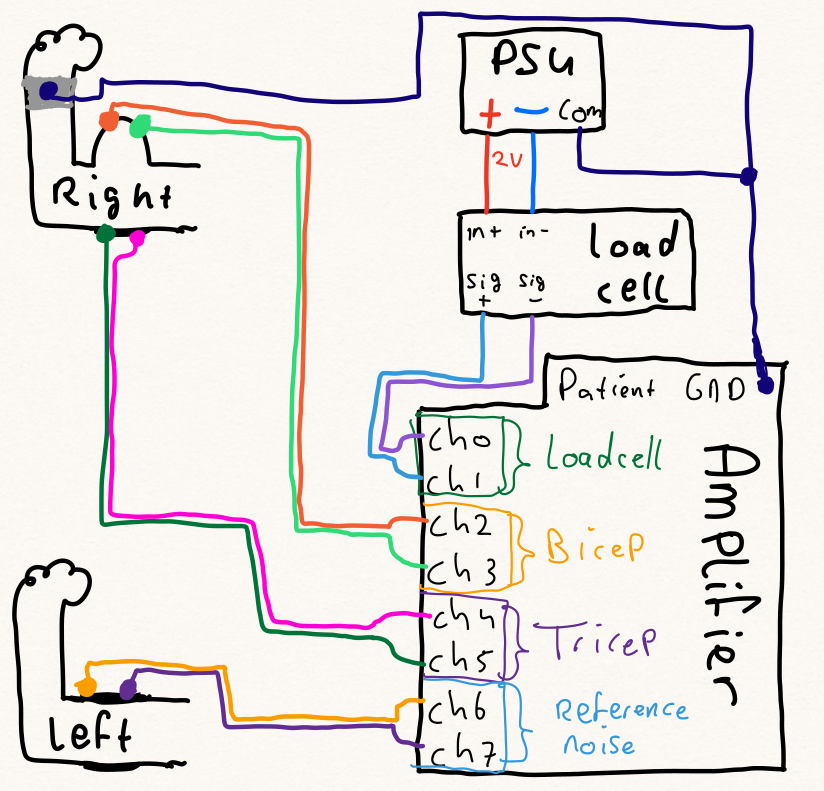
\includegraphics[width=1.0\columnwidth]{images/measurement_setup_diagram.png}
	\end{center}
	\caption{Diagram of the measurement setup}
	\label{fig:measurement_setup_diagram}
\end{figure}

\begin{figure}[h!t]
	\begin{center}
		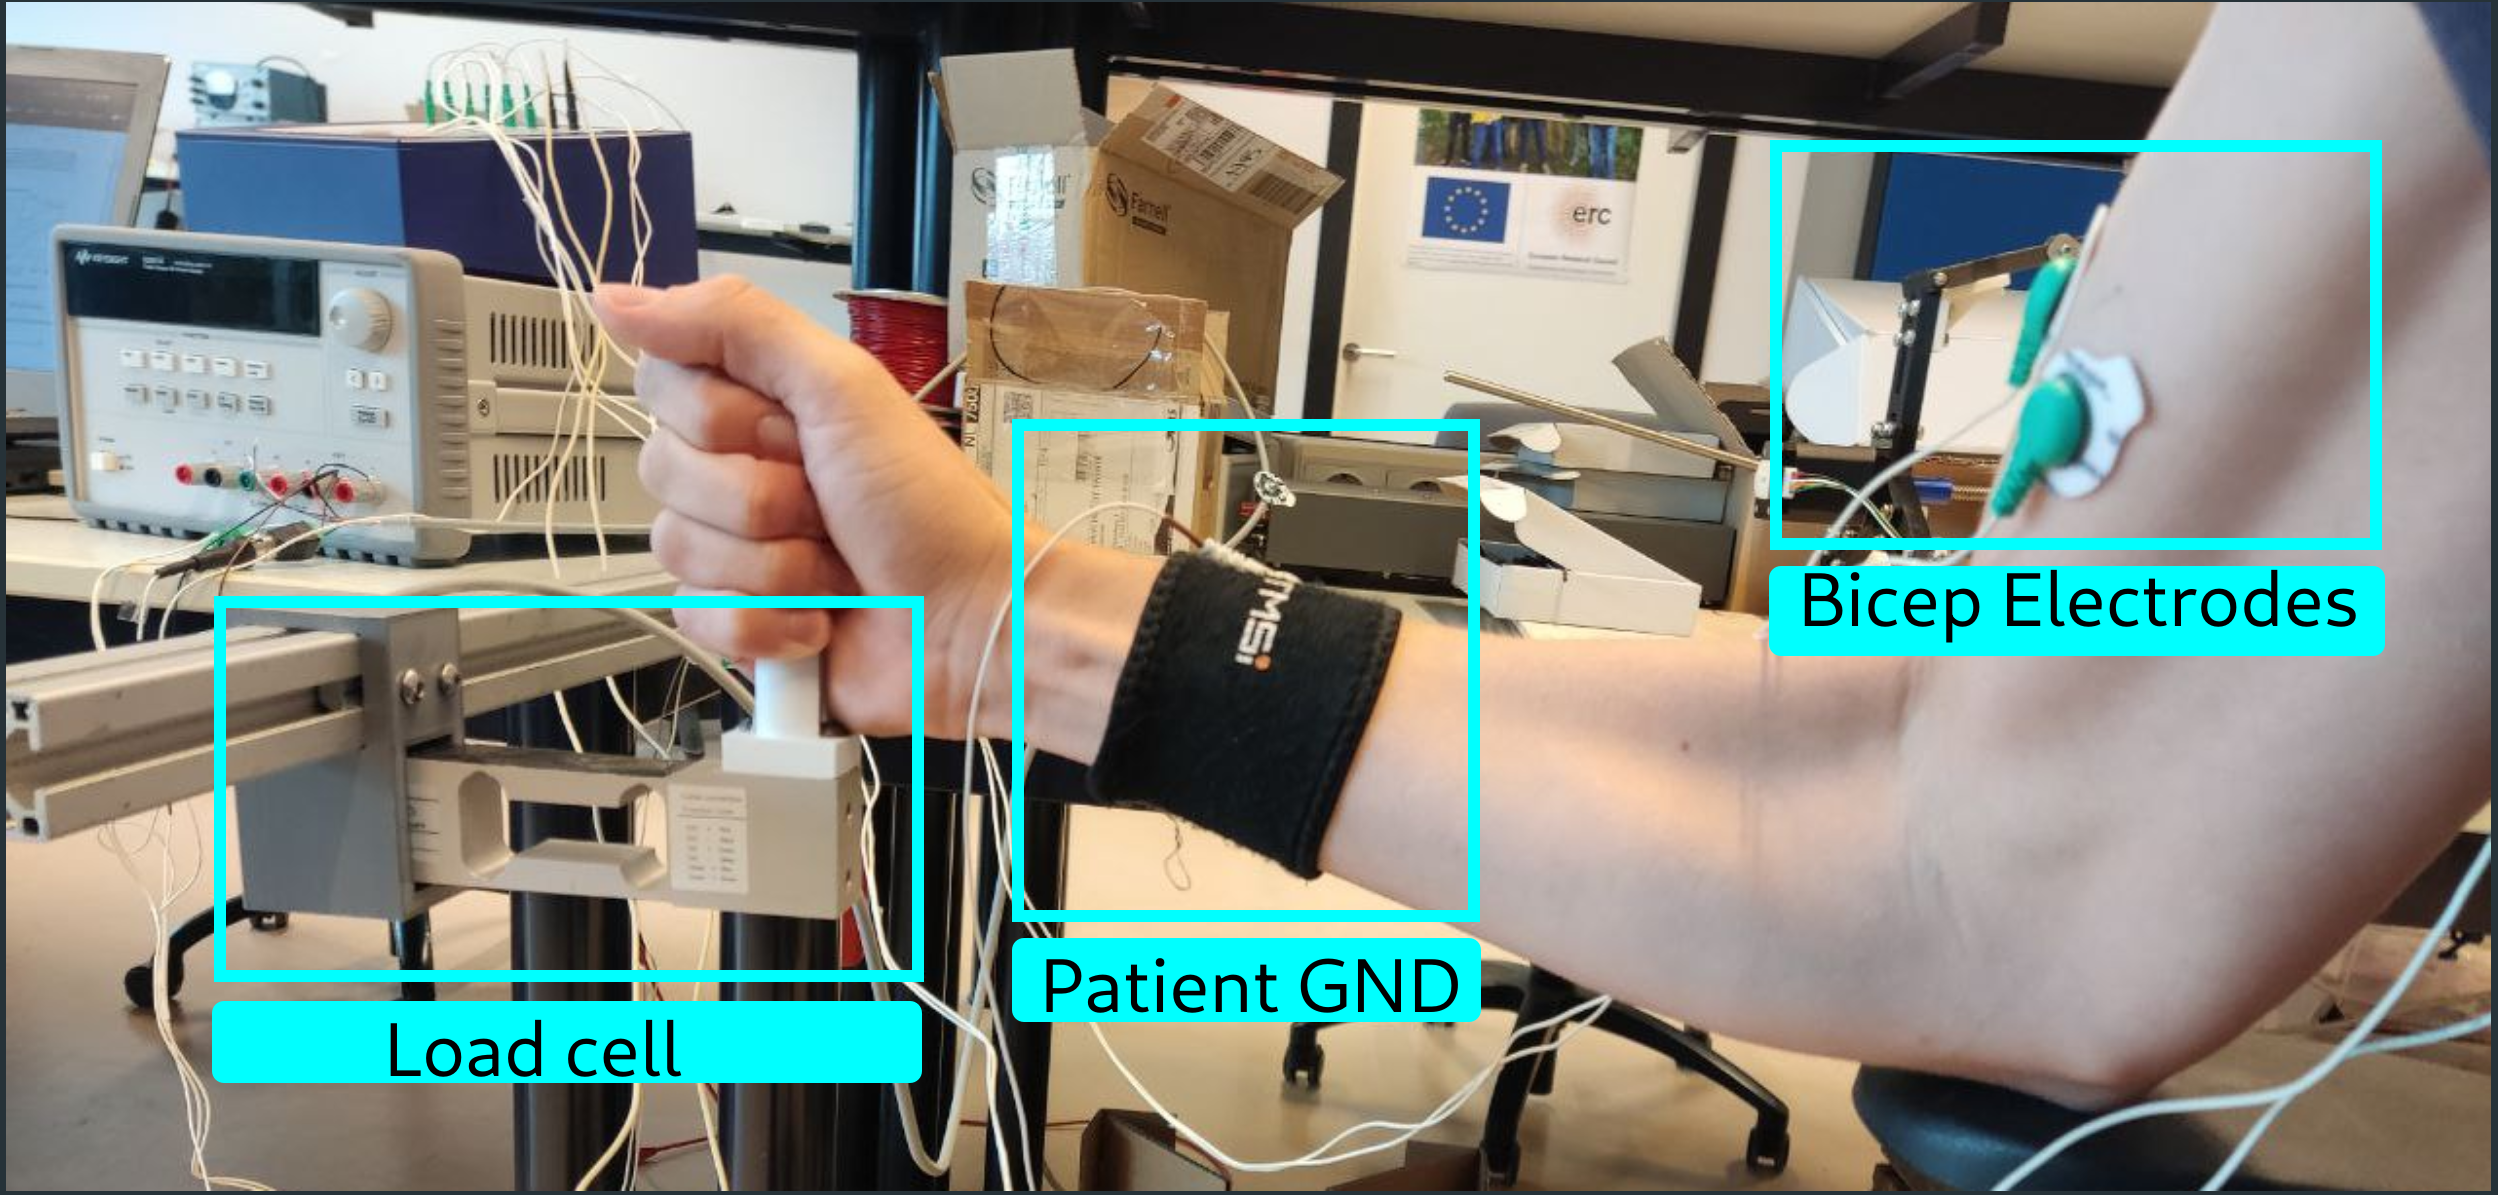
\includegraphics[width=1.0\columnwidth]{images/setup_photo.png}
	\end{center}
	\caption{Picture of the measurement setup}
	\label{fig:measurement_setup_photo}
\end{figure}

A single long measurement was taken at a sampling rate of \SI{1000}{\hertz} where force was applied following a predetermined pattern. This measurement is accompanied by a calibration measurements where an object with known weight was attached to the load cell at the sampling frequencies.

The applied force followed the following pattern:
\begin{itemize}
    \item Slowly pulling the handle upwards followed by a slow pushing the handle downwards. Repeated three times
    \item Slowly pull the load-cell upwards followed by returning to a neutral position. Repeated three times
    \item Slowly push the load-cell downwards followed by returning to a neutral position. Repeated three times
    \item Quickly pull the handle upwards followed by a quick push of the handle downwards. Repeated three times
\end{itemize}

\section{Measurement data}
The following configuration parameters were chosen based on simulation results:
\begin{itemize}
    \item Whitening: A whitening filter was created from the signal spectrum between 5 and 10 seconds in Figure~\ref{fig:measurement_1k}. The number of coefficients was limited to 500.
    \item Filtering
    \begin{itemize}
        \item Static filter: 3 notch filters at \SI{50}{\hertz}, \SI{100}{\hertz}, and \SI{150}{\hertz} with q-factor of 10, low-pass Butterworth filter with $f_{cut}$ of \SI{20}{\hertz} and length 5, high-pass Butterworth filter with $f_{cut}$ of \SI{300}{\hertz} and length 5
        \item Wiener filter: 200 filter terms, filter was created from the bicep signal
        \item Adaptive LMS filter: The filter length was 500 and the convergence value was 0.05
    \end{itemize}
    \item Envelope detection
    \begin{itemize}
        \item Moving average envelope detection: Length of filter was 120 terms
        \item IIR LP filter: $f_{cut}$ of \SI{4}{\hertz} and a filter order of 3
        \item RMS: Length of filter was 120 terms
    \end{itemize}
\end{itemize}


\begin{figure}[h!t]
	\begin{center}
		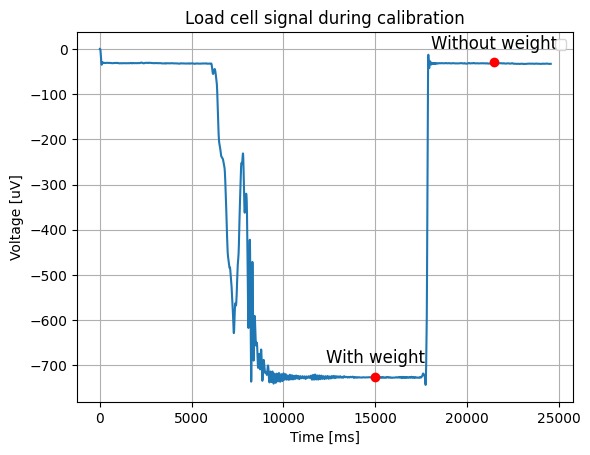
\includegraphics[width=0.8\columnwidth]{images/measurement_calibratie3_1k.png}
	\end{center}
	\caption{Calibration measurement at \SI{1}{\kilo\hertz} sampling rate. The force has been low-passed with an $f_{cut}$ of 10 Hz to remove large \SI{50}{\hertz} noise component. The offset was determined to be \SI{-30}{\micro\volt}. The weight op the object was \SI{1681}{\gram} which corresponds to a change of \SI{695}{\micro\volt}}.
	\label{fig:calibration_1k}
\end{figure}

\begin{figure}[h!t]
	\begin{center}
		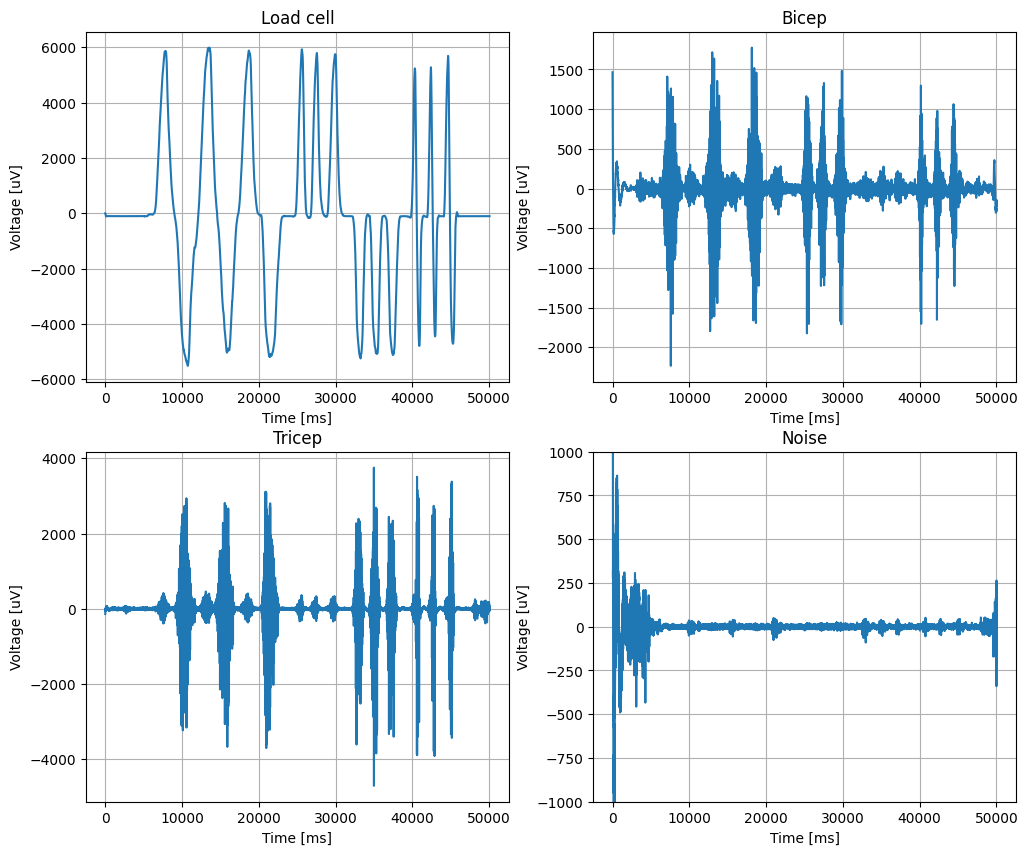
\includegraphics[width=1.0\columnwidth]{images/measurement_meting3_1k.png}
	\end{center}
	\caption{Force measurements and accompanying sEMG signals at \SI{1}{\kilo\hertz} sampling rate}
	\label{fig:measurement_1k}
\end{figure}

The calibration was performed to determine what the relation between the measured voltage and the force was. A weight of \SI{1681}{\gram} was attached to the measurement handle attached to the load cell which resulted in the measurement that can be seen in Figure~\ref{fig:calibration_1k}. Through visual inspection, the steady state offset of the setup without attached weight was determined to be \SI{30}{\micro\volt}. After attaching the weight, the steady state voltage was determined to be \SI{725}{\micro\volt}.

\begin{equation}
    \frac{\delta \text{weight [g]}}{\delta \text{signal [mV]}} = \frac{1681}{7.25-0.30} = 0.00241 [N/uV]
\end{equation}
The measured force in Newton is approximately 0.00241 times the measured signal in micro Volt.

All measurements were performed in bipolar electrode configuration and the measurement for a set of two electrodes was found by adding the results together. This removes the average signal that is present in all signals.

\section{Measurement processing result}
All combinations of whitening, filtering, and envelope detection were applied onto the signals as seen in Figure~\ref{fig:measurement_1k}. The combinations are indicated by the first letter of each processing method: 'w-s-r' means that Whitening was applied, the applied filter was a Static filter, and the envelope was determined using the RMS envelope detection. Further clarification can be found in Table~\ref{tab:abbreviation_explanation}.
During processing it was noticed that some methods scaled the estimated force by large amounts and this resulted in high error rates. To still compare the accuracy of force estimation regardless of scaling factor the decision was made to intrude an intermediate step between measuring/compensating the lag and calculating the error. After accounting for the lag, a scaling factor is determined that minimizes the RMSE. The scaling factor is determined through the following algorithm:
\begin{itemize}
    \item Calculate the RMSE
    \item Calculate the RMSE of a slightly amplified signal
    \item Calculate the RMSE of a slightly reduced signal
    \item Compare if amplifying or reducing the signal decreases the RMSE. If amplifying/reducing yields a lower RMSE, amplify/reduce the signal and repeat these steps. If amplifying and reducing both yield an RMSE lower than the current RMSE, the ideal scaling value has been found.
\end{itemize}

The estimated force is subsequently scaled by this scaling factor preparatory to calculating the RMSE value. For the RMSE calculation, the first 3 seconds and the last 3 seconds of the signals were discarded (after processing) because some processing steps did not yield their steady-state response in that time \cite{transient_response}. The results for lag, error, and scaling can be found in the bar-chart in Figure~\ref{fig:result_all_lagerrorscaling}. 

\begin{table} [h!]
\begin{tabular}{ccc}
Index & Abbreviation & Full form \\
\hline
0 & w/n & Whitening / No whitening \\
1 & n/s/w/a & No filter / Static filter / Wiener filter / Adaptive filter \\
2 & m/i/r & Moving average envelope / IIR LP envelope / RMS envelope \\
\end{tabular}
\caption{Table for clarifying the abbreviations used in result bar charts}
\label{tab:abbreviation_explanation}
\end{table}

\begin{figure}[h!t]
	\begin{center}
	\noindent\makebox[\textwidth]{
		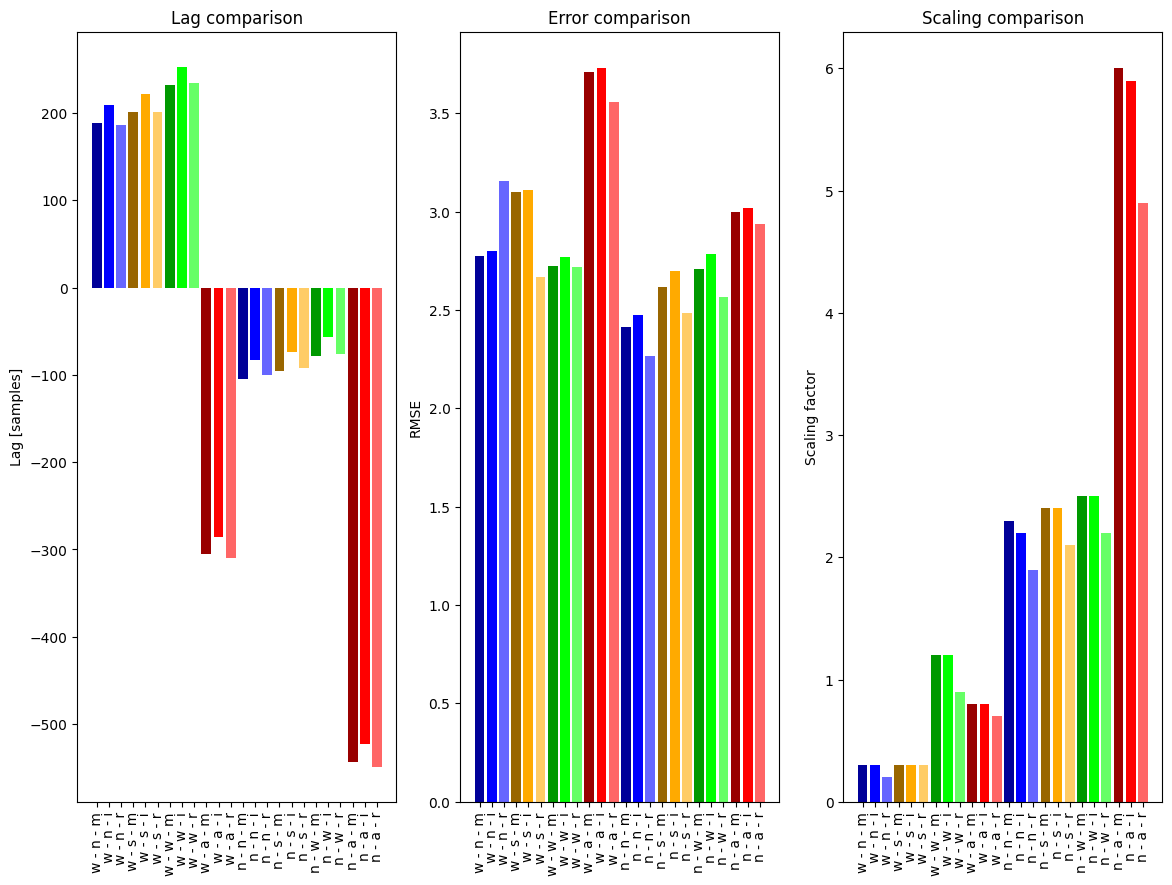
\includegraphics[width=1.3\columnwidth]{images/result_all_lagerrorscaling.png}}
	\end{center}
	\caption{This plot contains all relevant results for all different combinations of whitening, filters and envelope detection. The abbreviations are the first letter of the used technique for each step. Further clarification of these abbreviations can be found in Table~\ref{tab:abbreviation_explanation}}
	\label{fig:result_all_lagerrorscaling}
\end{figure}

\begin{figure}[h!t]
	\begin{center}
	\noindent\makebox[\textwidth]{
		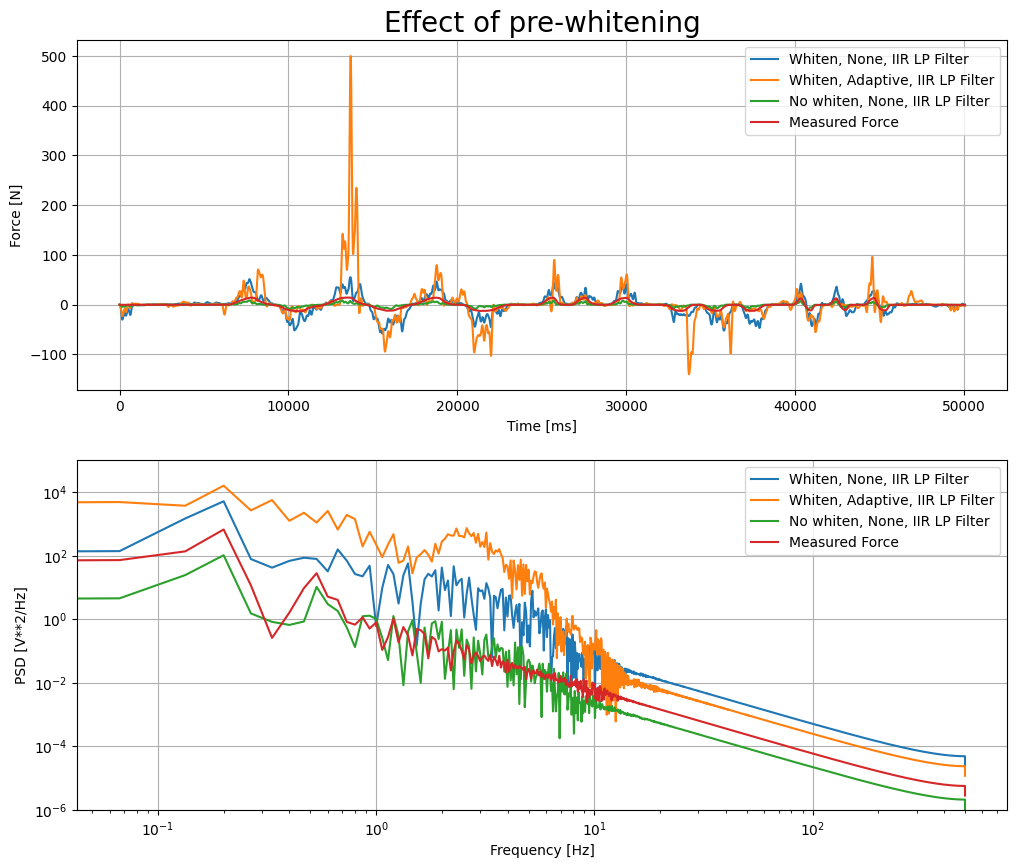
\includegraphics[width=1.3\columnwidth]{images/measurement_prewhitening.png}}
	\end{center}
	\caption{This figure illustrates the effect that whitening of the sEMG signal has on the resulting envelope. The signals were not filtered and moving average was used for envelope detection. Both unfiltered and adaptive filtered versions show volatile behaviour compared to the non-whitened variant. In the frequency domain it can be seen that whitening results in a spectrum of larger amplitude compared to the non-whitened spectrum which seems to follow the measured force much more closely}
	\label{fig:result_prewhitening}
\end{figure}


\begin{figure}[h!t]
	\begin{center}
		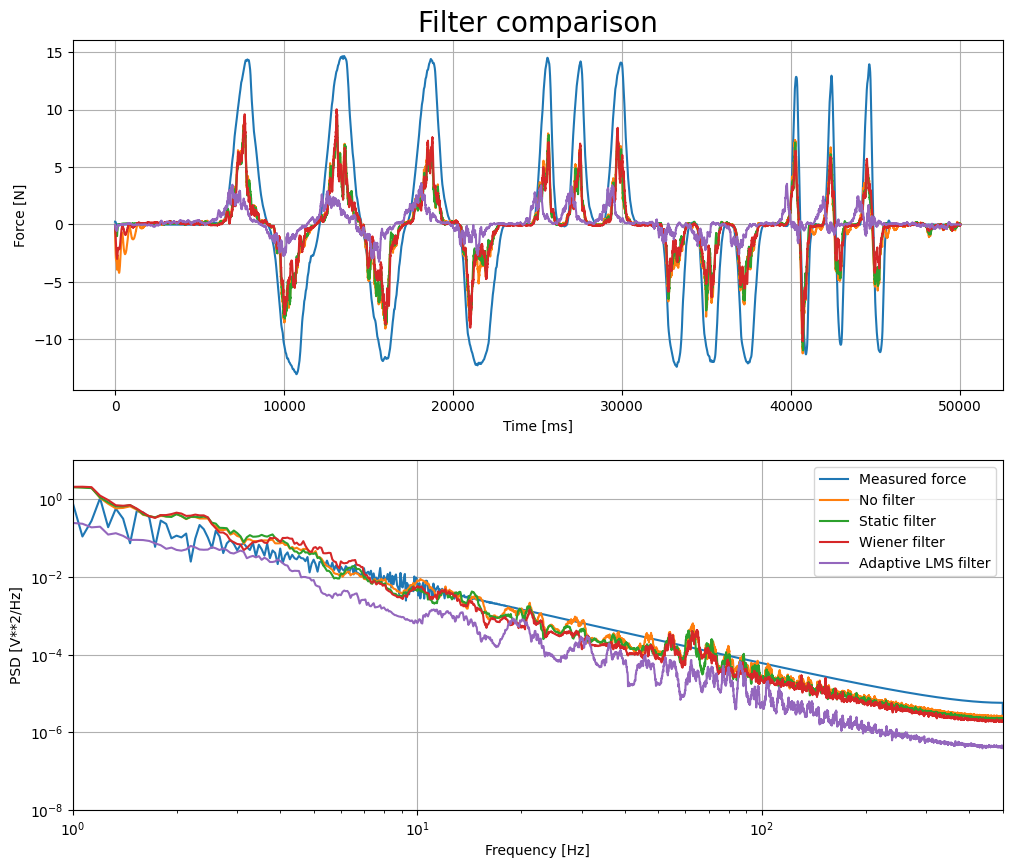
\includegraphics[width=1.0\columnwidth]{images/measurement_filtering.png}
	\end{center}
	\caption{This figure illustrates the effect that different filtering techniques have on the resulting envelope. The signals were not whitened and moving average was used for envelope detection. The frequency plots have been smoothed using a moving average filter of length 10 to clearer show the difference in behaviour. The volatile behaviour that the adaptive Wiener filter exhibits in the time domain matches the behaviour found in Figure~\ref{fig:result_prewhitening}}
	\label{fig:result_filtering}
\end{figure}


\begin{figure}[h!t]
	\begin{center}
		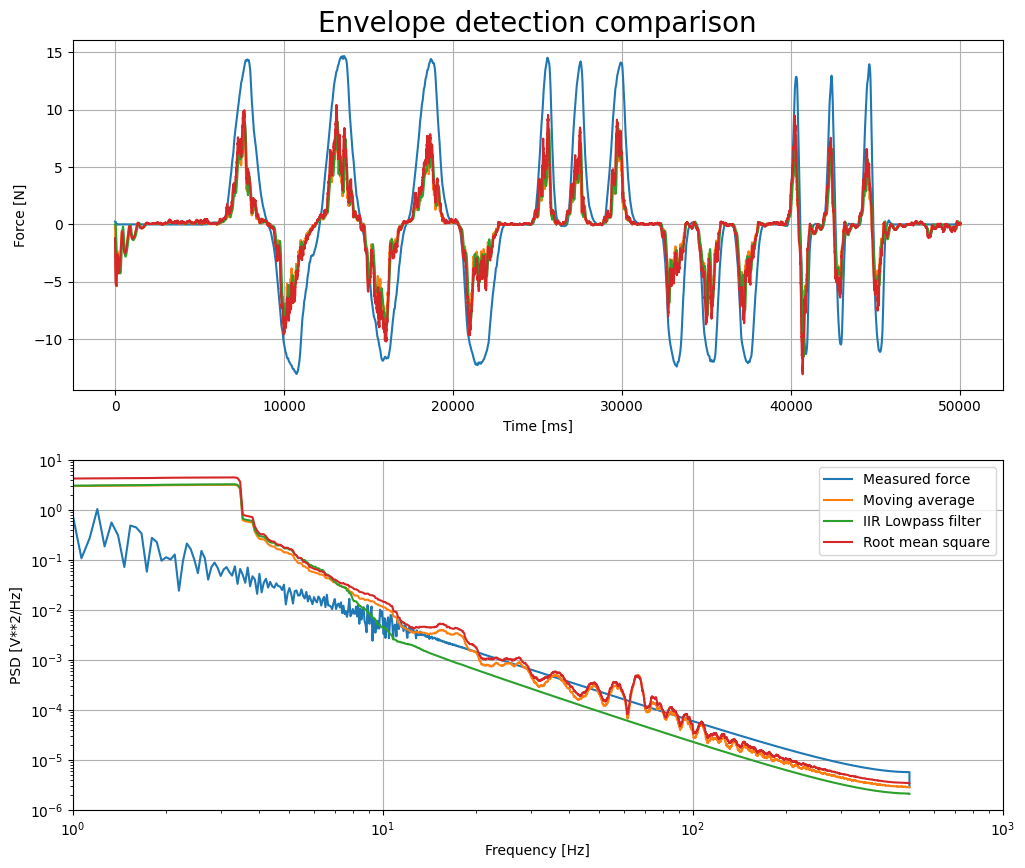
\includegraphics[width=1.0\columnwidth]{images/measurement_envelopes.png}
	\end{center}
	\caption{This figure illustrates the effect that different envelope estimation techniques have on sEMG signal. The signals were not whitened and not filtered. Even though all methods seem to provide almost identical behaviour in the time domain it can be seen from the frequency spectra that this only holds for moving average and root mean square envelope detection. IIR Butterworth low-pass filtering results in a more linear attenuation from the $f_{cut}$ on wards (set to 5Hz) which is in line with the simulations as seen in Figure~\ref{fig:iir_frequencyresponse_coefficients}}
	\label{fig:result_envelopes}
\end{figure}

\section{conclusion}